\begin{frame}
  \frametitle{Ring-Polymer Normal Modes}
  $\bullet\kern1ex$\textbf{Normal Modes:} -- the ring-polymer potential can be diagonalized 
  \begin{equation*}
    % \left.
    % \begin{gathered}
    %   \sum_{i=1}^P\frac{1}{2} m\omega_P^2(x_{i+1} - x_i)^2 \cr
    %   \tilde{x}_i = \sum_{j=1}^P x_j U_{ji}
    % \end{gathered}
    % \right\}
    \sum_{i=1}^P\frac{1}{2} m\omega_P^2(x_{i+1} - x_i)^2 
    % = \frac{1}{2}m\omega_P^2\mathbf{x}^T{\mathbf{A}}\mathbf{x}
    \quad\Longleftrightarrow\quad
    \begin{aligned}
        % \tilde{x}_k &= \sum_{j=1}^P x_j U_{jk} \cr
        \mathbf{\tilde{x}} &= \mathbf{U}\cdot \mathbf{x}\cr
        \mathbf{x} &= \mathbf{U}^T\!\!\cdot \mathbf{\tilde{x}}\cr
    \end{aligned}
    \quad\Longleftrightarrow\quad
    \sum_{j=1}^{P}\frac{1}{2} m\Omega_j^2\tilde{x}_j^2;
    % \quad
    % \Omega_j = 2\omega_P\sin(j\pi / P)
  \end{equation*}

  where $\mathbf{x}$ is the bead \textcolor{red}{Cartesian coordinate} and $\tilde{\mathbf{x}}$ is the \textcolor{blue}{normal mode}
  coordinate.

  \begin{multicols}{2}
    \begin{itemize}
        % \item $\tilde{x}_0 = (1/P)\sum_{i=1}^P x_i$ corresponds to the motion
        % of the centroid and $\Omega_0 = 0$.
        % \item $\tilde{x}_1 = (1/P)\sum_{i=1}^P x_i$ corresponds to the centroid.
        \item $\tilde{x}_1$ corresponds to the centroid motion and $\Omega_1 = 0$.
        \item The transformation $\mathbf{\tilde{x}} \Leftrightarrow \mathbf{x}$
          can be done with FFT.\footnote[frame]{
            \textit{J. Chem. Phys.}, \textbf{104}, 2028(1996).
          }
        \item The normal mode frequencies
        \footnote[frame]{
            This reminds me of the phonon dispersion of 1-D atomic chain.
            \smallskip
        }
        \begin{equation*}
            \Omega_j = 2\omega_P \sin\left({\frac{(j-1)\pi}{P}}\right)
        \end{equation*}

        e.g.\ $P = 8$
        \begin{center}
            % \resizebox{0.48\textwidth}{!}{
                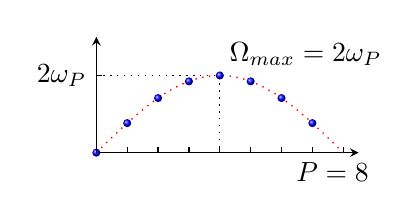
\begin{tikzpicture}
                [scale=0.98, x=0.4cm, y=1cm]
                \draw[->, >=stealth, black] (0.0, 0.0) -- (8.5, 0.0) node[below,pos=0.90] {$P = 8$};
                \draw[->, >=stealth, black] (0.0, 0.0) -- (0.0, 1.5) node[right] {
                    % \small $\Omega_j = 2\omega_P\sin(j\pi/P)$
                };
                \draw[line width=0.5pt, color=red, domain=0:8.0, dotted]
                    plot [samples=300] (\x, {sin(\x r * pi / 8)});

                \foreach \x in {0,1,...,7}{
                    \shade[ball color=blue] (\x, {sin(\x r * pi / 8)}) circle (1.5pt);
                }
                \foreach \x in {0, 1, ..., 8}{
                    \draw[line width=0.5pt] (\x, 0.0) node[below] {} -- ++(0.0, 2pt);
                }
                \draw[line width=0.5pt] (0.0, 1.0) node[left] {$2\omega_P$} -- ++(2pt, 0.0);
                \draw[line width=0.5pt, dotted] (0.0, 1.0) -- (4.0, 1.0) -- (4.0, 0.0);
                % \draw[>=stealth, ->] (4.0, 1.0) -- ++(0.0, -0.4) node[below] {$\Omega_{\text{max}} = 2\omega_P$};
                \node[above right] at (4.0, 1.0) {$\Omega_{\text{max}} = 2\omega_P$};
                \end{tikzpicture}
            % }
        \end{center}

        \item The matrix element $U_{kj}$ of the unitary transformation matrix $\mathbf{U}$ for even $P$

            \begin{equation*}
                % U_{jk} =
              \resizebox{1.0\linewidth}{!}{
                $\displaystyle
                \begin{cases}
                  \sqrt{1/P}, & k = 1 \\
                  \sqrt{2/P}\cos\left({2\pi\over P} (j-1)(k-1)\right), & 2 \le k \le P/2 \\
                  \sqrt{1/P}(-1)^j, & k = P / 2 + 1\\
                  \sqrt{2/P}\sin\left({2\pi\over P} (j-1)(k-1)\right), & P/2 + 2 \le k \le P
                \end{cases}
                $
              }
            \end{equation*}
          
            and $\tilde{x}_k = \sum_{j=1}^P U_{kj}x_j$.
          \item Note if we choose $\beta_P H_P \Rightarrow \beta (H_P/P)$, then
            \begin{align*}
                \mathbf{\tilde{x}} &= \frac{1}{\sqrt{P}} \,\mathbf{U} \cdot
                                     \mathbf{x} \cr
                \mathbf{x} &= \sqrt{P} \,\mathbf{U}^T \cdot
                                     \mathbf{\tilde{x}}
            \end{align*}
            

    \end{itemize}
    
  \end{multicols}

  % \begin{columns}
  %   \begin{column}{0.5\textwidth}
  %       \begin{itemize}
  %         % \item $\tilde{x}_0 = (1/P)\sum_{i=1}^P x_i$ corresponds to the centroid and $\Omega_0 = 0$.
  %         \item $\tilde{x}_0$ corresponds to the centroid and $\Omega_0 = 0$.
  %         \item The normal mode frequencies
  %           \footnote[frame]{
  %               This reminds me of the phonon dispersion of 1-D atomic chain.
  %           }
  %           \begin{equation*}
  %             \Omega_j = 2\omega_P \sin\left({\frac{(j-1)\pi}{P}}\right)
  %           \end{equation*}
            
  %         \item The unitary transformation matrix $\mathbf{U}$ for even $P$

  %           \begin{equation*}
  %             U_{jk} =
  %             \begin{cases}
  %               \sqrt{1/P}, & k = 1 \\
  %               \sqrt{2/P}\cos(2\pi jk /P), & 2 \le k \le P/2 \\
  %               \sqrt{1/P}(-1)^j, & k = P / 2 + 1\\
  %               \sqrt{2/P}\sin(2\pi jk /P), & P/2 + 2 \le k \le P
  %             \end{cases}
  %           \end{equation*}
            
  %       % \item For $P = 2n$, $\Omega_0 = 0$ and $\Omega_n = 2\omega_P$. 
  %       % \item For $P = 2n + 1$, $\Omega_0 =0$ and $\Omega_n = \omega_{P-n}$.
  %       \end{itemize}
  %   \end{column}
      
  %   \begin{column}{0.5\textwidth}
  %       \begin{figure}
  %           \centering
  %           \resizebox{1.00\textwidth}{!}{
  %               \begin{tikzpicture}
  %               [xscale=1.0, yscale=1.0]
  %               \draw[->, >=stealth, black] (0.0, 0.0) -- (8.5, 0.0) node[below] {$P = 7$};
  %               \draw[->, >=stealth, black] (0.0, 0.0) -- (0.0, 1.5) node[right] {
  %                   \small $\Omega_j = 2\omega_P\sin(j\pi/P)$
  %               };
  %               \draw[line width=0.5pt, color=red, domain=0:7.0, dotted]
  %                   plot [samples=300] (\x, {sin(\x r * pi / 7)});

  %               \foreach \x in {0,1,...,6}{
  %                   \shade[ball color=red] (\x, {sin(\x r * pi / 7)}) circle (1.5pt);
  %               }
  %               \foreach \x in {0, 1, ..., 8}{
  %                   \draw[line width=0.5pt] (\x, 0.0) node[below] {\x} -- ++(0.0, 2pt);
  %               }

  %               \draw[line width=0.5pt] (0.0, 1.0) node[left] {$2\omega_P$} -- ++(2pt, 0.0);
  %               \draw[line width=0.5pt, dotted] (0.0, 1.0) -- (3.5, 1.0) -- (3.5, 0.0);
  %               % \draw[line width=0.5pt] (4.0, 0.0) node[below] {\ldots} -- ++(0.0, 2pt);
  %               \end{tikzpicture}
  %           }

  %           \resizebox{1.00\textwidth}{!}{
  %               \begin{tikzpicture}
  %               \draw[->, >=stealth, black] (0.0, 0.0) -- (8.5, 0.0) node[below] {$P = 8$};
  %               \draw[->, >=stealth, black] (0.0, 0.0) -- (0.0, 1.5) node[right] {
  %                   % \small $\Omega_j = 2\omega_P\sin(j\pi/P)$
  %               };
  %               \draw[line width=0.5pt, color=red, domain=0:8.0, dotted]
  %                   plot [samples=300] (\x, {sin(\x r * pi / 8)});

  %               \foreach \x in {0,1,...,7}{
  %                   \shade[ball color=blue] (\x, {sin(\x r * pi / 8)}) circle (1.5pt);
  %               }
  %               \foreach \x in {0, 1, 2, ..., 8}{
  %                   \draw[line width=0.5pt] (\x, 0.0) node[below] {\x} -- ++(0.0, 2pt);
  %               }
  %               \draw[line width=0.5pt] (0.0, 1.0) node[left] {$2\omega_P$} -- ++(2pt, 0.0);
  %               \draw[line width=0.5pt, dotted] (0.0, 1.0) -- (4.0, 1.0) -- (4.0, 0.0);
  %               % \draw[>=stealth, ->] (4.0, 1.0) -- ++(0.0, -0.4) node[below] {$\Omega_{\text{max}} = 2\omega_P$};
  %               \node[above right] at (4.0, 1.0) {$\Omega_{\text{max}} = 2\omega_P$};
  %               \end{tikzpicture}
  %           }

  %           % \begin{tikzpicture}
  %           %   \draw[->, >=stealth, black] (0.0, 0.0) -- (8.5, 0.0) node[below] {$P$};
  %           %   \draw[->, >=stealth, black] (0.0, 0.0) -- (0.0, 1.5) node[right] {
  %           %     \small $\Omega_j = 2\omega_P\sin(j\pi/P)$
  %           %   };
  %           %   \draw[line width=0.5pt, color=blue, domain=0:7.0]
  %           %     plot [samples=300] (\x, {sin(\x r * pi / 7)});
  %           %   \draw[line width=0.5pt, color=red, domain=0:8.0]
  %           %     plot [samples=300] (\x, {sin(\x r * pi / 8)});

  %           %   \foreach \x in {0,1,...,7}{
  %           %     \draw[red] (\x, {sin(\x r * pi / 8)}) circle (2pt);
  %           %     \draw[blue] (\x, {sin(\x r * pi / 7)}) circle (2pt);
  %           %   }
  %           %   \foreach \x in {0, 1, 2, ..., 7}{
  %           %     \draw[line width=0.5pt] (\x, 0.0) node[below] {\x} -- ++(0.0, 2pt);
  %           %   }
  %           % \end{tikzpicture}
  %       \end{figure}
  %   \end{column}
  % \end{columns}
\end{frame}
